\skriptsection{Transformations (V2)}{104}
Transformation is done using the inverse transformation $T^{-1}$ which means that the loop is done 
in the output space and not in the input space. Otherwise, some holes or overlaps are possible.

\begin{minipage}{9cm}
  \skriptsubsection{Affine Transformations}{87}
  $[x \; y] = [w \; z] \begin{bmatrix}
  a_{11} &a_{12} \\ a_{21} &a_{22}
  \end{bmatrix} + [b_1 \; b_2]$
  
  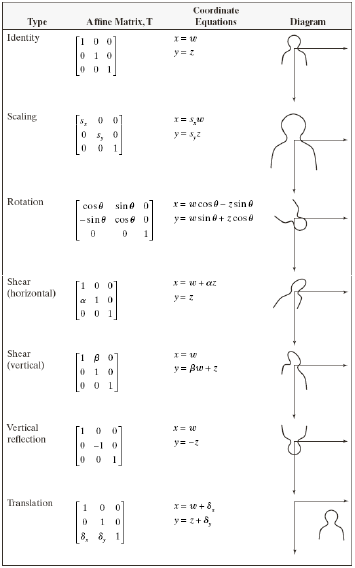
\includegraphics[width=7cm]{./images/affine_transformations.png}
\end{minipage}
\begin{minipage}{9cm}
  \skriptsubsection{Interpolation}{65}
  Methods: Nearest Neighbour; Bilinear (image); Bicubic\\
  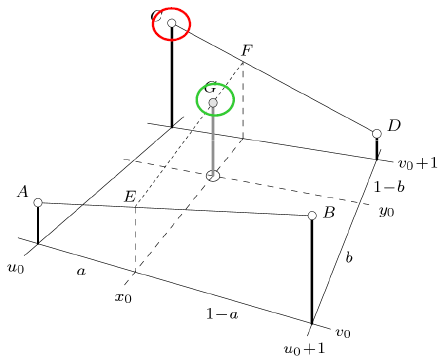
\includegraphics[width=7cm]{./images/bilinear_interpolation.png}
  
  \subsection{Image Registration}
  Image registration is the process of aligning (multiple) images or bringing them into one coordinate 
  system geometrically.
  \begin{itemize}
    \item Feature extraction
    \item Find transform to reference image
    \item Transform image
  \end{itemize}
\end{minipage}

